%% For normal draft builds (figs undisplayed hence fast compile)
%\documentclass[hyperpdf,nobind,draft,oneside]{hepthesis}
%\documentclass[hyperpdf,nobind,draft,twoside]{hepthesis}

%% For short draft builds (breaks citations by necessity)
%documentclass[hyperpdf,nobind,draft,hidefrontback]{hepthesis}

%%For Cambridge soft-bound version
%\documentclass[hyperpdf,bindnopdf]{hepthesis}
%% For Cambridge hard-bound version (must be one-sided)
%\documentclass[hyperpdf,oneside]{hepthesis}
%%Get rid of warnings about list of figures and tables but also remove from ToC
\documentclass[hyperpdf,oneside,notlot,notlof]{hepthesis}

%% Load special font packages here if you wish
%\usepackage{lmodern}
%\usepackage{mathpazo}
%\usepackage{euler}

%% Put package includes etc. into preamble.tex for convenience
\usepackage{xspace}
\usepackage{tikz}
\usepackage{morefloats,afterpage}
\usepackage{mathrsfs} % script font
\usepackage{verbatim}
\usepackage{multirow}
\usepackage{nicematrix}
\usepackage{lipsum}
\usepackage{feynman}
\usepackage{adjustbox}
\usepackage{arydshln}
\usepackage{subcaption}
\usepackage[utf8]{inputenc}
\usepackage{amsmath}
\usepackage{amsfonts}
\usepackage{amssymb}
\usepackage{fullpage}
\usepackage{lscape}
\usetikzlibrary{angles, quotes}
\usepackage{parskip}
\pdfminorversion=6
\usepackage{url}

%\usepackage{indentfirst}
\usepackage[en-GB]{datetime2}
\makeatletter
\newcommand{\monthyeardate}{%
  \DTMenglishmonthname{\@dtm@month}, \@dtm@year
}
\makeatother

\usepackage[a4paper,
            left=40mm,
            right=25mm]{geometry}

% glossary - add to toc and remove page numbers
\usepackage[xindy,toc,nonumberlist]{glossaries-extra} 
\setabbreviationstyle[acronym]{long-short}
\makeglossaries
%\newglossaryentry{domain-knowledge}{%
%  name={domain knowledge},%
%  description={valid knowledge used to refer to an area of human endeavour, an autonomous computer activity, or other specialized discipline}}

\newacronym{adc}{ADC}{Analog Digital Converter}
\newacronym{apa}{APA}{Andode Plane Assembly}
\newacronym{arapuca}{ARAPUCA}{Argon R\&D Advanced Program at UniCAmp}
\newacronym{argoneut}{ArgoNeuT}{Argon Neutrino Test Stand}
\newacronym{bnb}{BNB}{Booster Neutrino Beam}
\newacronym{bsm}{BSM}{Beyond Standard Model}
\newacronym{cc}{CC}{Charged Current}
\newacronym{ccqe}{CCQE}{Charged Current Quasi Elastic}
\newacronym{cp}{CP}{charge-parity}
\newacronym{cpa}{CPA}{Cathode Plane Assembly}
\newacronym{crt}{CRT}{Cosmic Ray Tagger}
\newacronym{donut}{DONUT}{Direct Observation of the Nu Tau}
\newacronym{dune}{DUNE}{Deep Underground Neutrino Experiment}
\newacronym{em}{EM}{electromagnetic}
\newacronym{es}{ES}{Elastic Scattering}
\newacronym{fermilab}{Fermilab}{Fermi National Accelerator Laboratory}
\newacronym{fnal}{FNAL}{Fermi National Accelerator Laboratory}
\newacronym{gallex}{GALLEX}{Gallium Experiment}
\newacronym{icarus}{ICARUS}{Imaging Cosmic and Rare Underground Signals}
\newacronym{karmen}{KARMEN}{Karlsruhe Rutherford Medium Energy Neutrino}
\newacronym{larsoft}{LArSoft}{Liquid Argon Software}
\newacronym{lartpc}{LArTPC}{Liquid Argon Time Projection Chamber}
\newacronym{lep}{LEP}{Large Electron-Positron Collider}
\newacronym{lsnd}{LSND}{Liquid Scintillator Neutrino Detector}
\newacronym{mc}{MC}{Monte Carlo}
\newacronym{microboone}{MicroBooNE}{Micro Booster Neutrino Experiment}
\newacronym{miniboone}{MiniBooNE}{Mini Booster Neutrino Experiment}
\newacronym{minos}{MINOS}{Main Injector Neutrino Oscillation Search}
\newacronym{mip}{MIP}{Minimum Ionising Particle}
\newacronym{nc}{NC}{Neutral Current}
\newacronym{nist}{NIST}{National Institute of Standards and Technology}
\newacronym{p}{P}{parity}
\newacronym{pdg}{PDG}{Particle Data Group}
\newacronym{pds}{PDS}{Photon Detection System}
\newacronym{pmns}{PMNS}{Pontecorvo-Maki-Nakagawa-Sakata}
\newacronym{pmt}{PMT}{Photo Multiplier Tube}
\newacronym{sage}{SAGE}{Soviet-American Gallium Experiment}
\newacronym{sbn}{SBN}{Short Baseline Neutrino}
\newacronym{sbnd}{SBND}{Short Baseline Near Detector}
\newacronym{sce}{SCE}{Space Charge Effect}
\newacronym{sipm}{SiPM}{Silicon Photomultiplier}
\newacronym{sk}{SK}{Super Kamiokande}
\newacronym{sm}{SM}{Standard Model}
\newacronym{sno}{SNO}{Sudbury Neutrino Observatory}
\newacronym{sp}{SP}{Space Point}
\newacronym{tla}{TLA}{Three Letter Acronym}
\newacronym{tpb}{TPB}{Tetraphenyl Butadiene}
\newacronym{tpc}{TPC}{Time Projection Chamber}
\newacronym{vuv}{VUV}{Vacuum Ultra Violet}







\glssetcategoryattribute{acronym}{glossname}{firstuc}
\glssetcategoryattribute{acronym}{glossdesc}{title}

% add line numbers
%\usepackage{lineno}
%\linenumbers

% redefine the \paragraph command so it acts like subsubsubsection
\RedeclareSectionCommand[runin=false,afterskip=1ex,afterindent=false]{paragraph}

% sort out the captions
\captionsetup{width = \textwidth}
\captionsetup{format = plain} %

% Define change margin command
\def\changemargin#1#2{\list{}{\rightmargin#2\leftmargin#1}\item[]}
\let\endchangemargin=\endlist 

%% Using Babel allows other languages to be used and mixed-in easily
%\usepackage[ngerman,english]{babel}
\usepackage[english]{babel}
\selectlanguage{english}

%% Citation system tweaks
\usepackage{cite}
% \let\@OldCite\cite
% \renewcommand{\cite}[1]{\mbox{\!\!\!\@OldCite{#1}}}

%% Maths
% TODO: rework or eliminate maybemath
\usepackage{abmath}
\DeclareRobustCommand{\mymath}[1]{\ensuremath{\maybebmsf{#1}}}
% \DeclareRobustCommand{\parenths}[1]{\mymath{\left({#1}\right)}\xspace}
% \DeclareRobustCommand{\braces}[1]{\mymath{\left\{{#1}\right\}}\xspace}
% \DeclareRobustCommand{\angles}[1]{\mymath{\left\langle{#1}\right\rangle}\xspace}
% \DeclareRobustCommand{\sqbracs}[1]{\mymath{\left[{#1}\right]}\xspace}
% \DeclareRobustCommand{\mods}[1]{\mymath{\left\lvert{#1}\right\rvert}\xspace}
% \DeclareRobustCommand{\modsq}[1]{\mymath{\mods{#1}^2}\xspace}
% \DeclareRobustCommand{\dblmods}[1]{\mymath{\left\lVert{#1}\right\rVert}\xspace}
% \DeclareRobustCommand{\expOf}[1]{\mymath{\exp{\!\parenths{#1}}}\xspace}
% \DeclareRobustCommand{\eexp}[1]{\mymath{e^{#1}}\xspace}
% \DeclareRobustCommand{\plusquad}{\mymath{\oplus}\xspace}
% \DeclareRobustCommand{\logOf}[1]{\mymath{\log\!\parenths{#1}}\xspace}
% \DeclareRobustCommand{\lnOf}[1]{\mymath{\ln\!\parenths{#1}}\xspace}
% \DeclareRobustCommand{\ofOrder}[1]{\mymath{\mathcal{O}\parenths{#1}}\xspace}
% \DeclareRobustCommand{\SOgroup}[1]{\mymath{\mathup{SO}\parenths{#1}}\xspace}
% \DeclareRobustCommand{\SUgroup}[1]{\mymath{\mathup{SU}\parenths{#1}}\xspace}
% \DeclareRobustCommand{\Ugroup}[1]{\mymath{\mathup{U}\parenths{#1}}\xspace}
% \DeclareRobustCommand{\I}[1]{\mymath{\mathrm{i}}\xspace}
% \DeclareRobustCommand{\colvector}[1]{\mymath{\begin{pmatrix}#1\end{pmatrix}}\xspace}
\DeclareRobustCommand{\Rate}{\mymath{\Gamma}\xspace}
\DeclareRobustCommand{\RateOf}[1]{\mymath{\Gamma}\parenths{#1}\xspace}

%% High-energy physics stuff
\usepackage{abhep}
\usepackage{hepnames}
\usepackage{hepunits}
\DeclareRobustCommand{\arXivCode}[1]{arXiv:#1}
\DeclareRobustCommand{\CP}{\ensuremath{\mathcal{CP}}\xspace}
\DeclareRobustCommand{\CPviolation}{\CP-violation\xspace}
\DeclareRobustCommand{\CPv}{\CPviolation}
\DeclareRobustCommand{\LHCb}{LHCb\xspace}
\DeclareRobustCommand{\LHC}{LHC\xspace}
\DeclareRobustCommand{\LEP}{LEP\xspace}
\DeclareRobustCommand{\CERN}{CERN\xspace}
\DeclareRobustCommand{\bphysics}{\Pbottom-physics\xspace}
\DeclareRobustCommand{\bhadron}{\Pbottom-hadron\xspace}
\DeclareRobustCommand{\Bmeson}{\PB-meson\xspace}
\DeclareRobustCommand{\bbaryon}{\Pbottom-baryon\xspace}
\DeclareRobustCommand{\Bdecay}{\PB-decay\xspace}
\DeclareRobustCommand{\bdecay}{\Pbottom-decay\xspace}
\DeclareRobustCommand{\BToKPi}{\HepProcess{ \PB \to \PK \Ppi }\xspace}
\DeclareRobustCommand{\BToPiPi}{\HepProcess{ \PB \to \Ppi \Ppi }\xspace}
\DeclareRobustCommand{\BToKK}{\HepProcess{ \PB \to \PK \PK }\xspace}
\DeclareRobustCommand{\BToRhoPi}{\HepProcess{ \PB \to \Prho \Ppi }\xspace}
\DeclareRobustCommand{\BToRhoRho}{\HepProcess{ \PB \to \Prho \Prho }\xspace}
\DeclareRobustCommand{\X}{\thesismath{X}\xspace}
\DeclareRobustCommand{\Xbar}{\thesismath{\overline{X}}\xspace}
\DeclareRobustCommand{\Xzero}{\HepGenParticle{X}{}{0}\xspace}
\DeclareRobustCommand{\Xzerobar}{\HepGenAntiParticle{X}{}{0}\xspace}
\DeclareRobustCommand{\epluseminus}{\Ppositron\!\Pelectron\xspace}
\DeclareRobustCommand{\protonproton}{\Pproton\APantiproton\xspace}


%% You can set the line spacing this way
%\setallspacing{double}
%% or a section at a time like this
%\setfrontmatterspacing{double}


%% Define the thesis title and author
\title{Search for Sterile Neutrinos at the Short Baseline Neutrino Program}
\author{Thomas Ham}

%% Doc-specific PDF metadata
\makeatletter
\@ifpackageloaded{hyperref}{%
\hypersetup{%
  pdftitle = {Search for Sterile Neutrinos at the SBN program},
  pdfsubject = {Andy Buckley's PhD thesis},
  pdfkeywords = {LHCb, B, physics, LHC, heavy flavour},
  pdfauthor = {\textcopyright\ Thomas Ham}
}}{}
\makeatother

% Redeclare the \EquationRef command so it uses \ref instead of \eqnref
\DeclareRobustCommand{\EquationRef}{Equation \ref}

%% Start the document
\begin{document}

%% Define the un-numbered front matter (cover pages, rubrik and table of contents)
\begin{frontmatter}
  %% Title
%\DTMlangsetup[en-US]{showyear=false}

\begin{comment}
\titlepage[\phantom{This text will be invisible} \\ 
\monthyeardate]
{%
\begin{figure}[h!]
    \centering
    
\includegraphics[width = 0.3\smallfigwidth]{figures-coat_of_arms/Arms_of_the_University_of_Liverpool.pdf}
\end{figure}
Thesis submitted in accordance with the requirements of the University of Liverpool for the degree of Doctor in Philosophy}
\end{comment}

%% Abstract
\setabstractextramargins{0cm}
\begin{abstract}%[\smaller \thetitle\\ \vspace*{1cm} \smaller {\theauthor}]
  %\thispagestyle{empty}

The \gls{sbn} program is comprised of three Liquid Argon Time Projection Chamber detectors located along the beam line of the Booster Neutrino Beam at Fermilab. The three detectors are SBND, MicroBooNE and ICARUS and are at 110 m, 470 m and 600 m from the beam source respectively. The program was designed with the goal of either confirming or refuting the existence of light sterile neutrinos, which have been hinted at by the LSND and MiniBooNE experiments as well as results from reactor and gallium based neutrino experiments. The observation of sterile neutrinos would provide physics beyond the Standard Model as well as being a vital component in understanding the mass generation mechanism for neutrinos. One of the defining properties of sterile neutrinos is that they do not weakly interact meaning that direct detection is not viable, however, mixing may occur with the active neutrinos which allows for the appearance and disappearance of active neutrinos to be observed.  

The development of electromagnetic shower reconstruction algorithms used in SBND are presented which are crucial for calculating the reconstructed neutrino energy from \nue CC interactions. The neutrino energy is one of the variables used to calculate the neutrino oscillation probability which is the other major topic that is discussed in this thesis. Assuming a $(3+1)$ neutrino framework, the \nue appearance and disappearance sensitivities are calculated from a \nue CC inclusive sample for the SBN program using Monte Carlo events. %The analysis included flux and interaction systematic parameters as well as a discussion on the possible impact due to efficiency uncertainties. 
The \nue appearance exclusion sensitivities from SBND show a stronger constraint than previous results and the allowed region is compatible with the LSND result. The SBN \nue disappearance exclusion sensitivity excludes much of the allowed region from the ND280 detector whereas the SBN allowed region is still compatible with that from ND280.
\end{abstract}

%% Add Glossary
\glsaddall 
\glsunsetall

%% Declaration
\setdeclarationextramargins{0cm}
\begin{declaration}
  
  I hereby confirm this work is my own, except where other works are referenced. This work has not previously been submitted to any institute, including this one.
  
  \ChapterRef{chap:Introduction} gives an overview of the content in this thesis. \ChapterRef{chap:Neutrino Physics} and \ChapterRef{chap:SBN Program} give a review of neutrino theory and details of neutrino detection using \glspl{lartpc} with a focus on the key features of the \gls{sbn} program. These chapters cover work done by many members of the wider neutrino community and have been referenced where appropriate. 
  
  \ChapterRef{chap:Energy_Reco} builds upon the reconstruction work done by a number of people as part of the \gls{larsoft} framework. In particular, the \textit{Shower Num Electrons Energy tool} and the \textit{Shower ESTAR Energy tool} have been newly developed and validated by myself.
  
  \ChapterRef{chap:osc_inputs} discusses the necessary inputs and analysis choices required for a sterile neutrino oscillation analysis. Again, many people worked on different aspects of the work presented here. Personally, I produced the most recent \nue \gls{mc} event sample and performed the study investigating the impact of the baseline parametrisation. \ChapterRef{chap:VALOR} goes on to use the inputs from \ChapterRef{chap:osc_inputs} to perform an oscillation analysis using the VALOR fitting framework. The content shown is essentially all my own and builds upon the work done by current and previous members of the VALOR group. 
  
  \begin{comment}
  Chapters 2 - Historical neutrino overview, obviously not my own work. \\
  Chapter 3 - LArTPC physics and SBN program overview. Small contribution to work on the PDS system, otherwise not my work. \\
  Chapter 4 - Many people work on Larsoft / Reconstruction. Shower Linear Energy tool originally worked on by Dom. Other two tools developed by me. \\
  Chapter 5 - \nue event production and selection is work done by Dom (and Gray?), however, the most recent events sample were produced by me using their work. GENIE/miniboone systematics is work done by SOMEONE?. Detector systematics developed by VALOR group. Baseline approximation done by steve/dom. Impact of baseline studies done by me. \\
  Chapter 6 - VALOR intially develped by Costas et. al. \nue stuff all done by me. Rhiannon did \numu. Impact of detector systematics all done by moi. 
  
  %\begin{flushright}
  %  Name??
  %\end{flushright}
  \end{comment}
\end{declaration}

%% Acknowledgements
\begin{acknowledgements}
    
  Firstly, I would like to thank Costas for your continued support and general guidance over the past four years, but in particular, for the role you played in leading the VALOR group. Naturally, the VALOR group consists of members, past and present, many of whom have provided valuable contributions to my PhD in one way or another. 
  
  I would also like to thank Dom Brailsford and Ornella (and the numerous other SBN members who are associated with Larsoft and reconstruction work). You have both engaged in insightful discussions and helped in the development and validation of the EM shower reconstruction algorithms. 

  Finally, the Liverpool student cohort deserves a mention and a thank you for providing an entertaining social aspect to my time here. 

\end{acknowledgements}

%% Preface
%\begin{preface}
%  Preface??
%\end{preface}

%% ToC
% set sectioning levels - 3 = subsubsection
\setcounter{tocdepth}{3}
\setcounter{secnumdepth}{3}
\tableofcontents



%% Strictly optional!
%\frontquote{%
%  Writing in English is the most ingenious torture\\
%  ever devised for sins committed in previous lives.}%
%  {James Joyce}
%% I don't want a page number on the following blank page either.
\thispagestyle{empty}


\printglossaries

% Have the short form for glossary entries in the list of tables and figures
\glsunsetall

%% I prefer to put these tables here rather than making the
%% front matter seemingly interminable. No-one cares, anyway!

% Rename the "List of ..." in the ToC.
\renewcommand{\listfigurename}{List of Figures}
\renewcommand{\listtablename}{List of Tables}

\listoffigures
\listoftables

% Reset the glossary so the definitions start after list of tables and figures
\glsresetall




\end{frontmatter}

%% Start the content body of the thesis
\begin{mainmatter}
  %% Actually, more semantic chapter filenames are better, like "chap-bgtheory.tex"
  %\chapter{Introduction}
\label{chap:Introduction}

%% Restart the numbering to make sure that this is definitely page #1!
\pagenumbering{arabic}

Neutrinos are a class of neutral leptonic particle that, within the \gls{sm}, only interact via the weak interaction and gravity \cite{Particles_and_Fundamental_Interactions:_An_Introduction_to_Particle_Physics}. The idea of a neutrino was first proposed in 1930 by Pauli and was not experimentally confirmed until 1956 by Cowan and Reines \cite{Pauli_letter} \cite{cowan_and_reines_paper}. Two further types (or flavours) of neutrinos were discovered in 1962 and 2000 by the Alternating Gradient Synchrotron and the \Gls{donut} experiment respectively \cite{Muon_neutrino_discovery} \cite{DONUT}. 

Neutrinos were long thought to be massless, but results from the \gls{sk} collaboration in 1988 showed that the flavour of a neutrino may oscillate which disabused this idea \cite{SuperK_neutrino_oscillations}. Confirmation of neutrino oscillations required non-zero neutrino masses and also helped resolve the long standing \textit{Solar Neutrino Problem} and the \textit{Atmospheric Neutrino Anomaly} \cite{Homestake} \cite{Atmospheric_anomaly}. There are, however, still a number of open questions which are of interest to particle physics that are linked to neutrinos, such as; 
\begin{itemize}
    \item The amount, if any, of \gls{cp} violation in the lepton sector.
    \item The absolute mass of the neutrinos.
    \item The neutrino mass hierarchy. 
    \item The Dirac or Majorana nature of neutrinos. Since neutrinos are neutral particles, it is possible that they may be their own anti-particles (a Majorana particle), a property that would be unique to neutrinos. 
    \item The possible existence of sterile neutrinos which are additional flavours of neutrinos that would only interact via gravity. 
\end{itemize}
The Majorana nature of neutrinos would allow for neutrinoless double beta decay, a process which does not conserve lepton number \cite{neutrinoless_double_beta_decay}. Sterile neutrinos have been hinted at by a number of experiments and are expected to have right handed helicities which is in contrast to the active neutrinos which have all been observed to have left handed helicities \cite{White_Paper}. The confirmation of either of these would give direct evidence of physics beyond the \gls{sm}. All of these question are under active investigation by current and future neutrino experiments. 

The focus of this thesis will be on the \gls{sbn} program which is currently under development with the main goal being to either confirm or refute the existence of light sterile neutrinos. The \gls{sbn} program is located at Fermilab and consists of three distinct \gls{lartpc} type detectors located along the \gls{bnb} beamline \cite{SBN_Proposal}. The \gls{sbnd} will be the nearest detector to the beam source at a distance of a 110 m and is currently under construction with the expectation that data taking will begin in early 2024 \cite{sbnd_timeline}. The two other detectors which are part of the \gls{sbn} program are the \gls{microboone} detector at 470 m and the \gls{icarus} detector at 600 m from the beam source, both of which are currently taking data. As mentioned, the main goal of the program will be to search for eV scale sterile neutrinos, but there are numerous other aims which include, measuring neutrino-argon interactions (due to the close proximity of \gls{sbnd} to the beam source, the observed statistics will far exceed that of any current dataset), developing large scale \gls{lartpc} technology and the search for possible \gls{bsm} processes \cite{SBN_paper}. All of these will be crucial in the development and physics analysis of future \gls{lar} neutrino detectors such as the \gls{dune}. 

The remaining content of this thesis begins with \ChapterRef{chap:Neutrino Physics}, which gives a brief overview of the ideas and experiments which have lead to the discovery of the three active neutrino flavours. This is then followed by a discussion of the key physics principles describing neutrino behaviour. Finally, the experimental results which are at odds with a 3 flavour paradigm and point towards the presence of sterile neutrinos are considered along with the theory that underpins their possible existence. 

\ChapterRef{chap:SBN Program} then gives an overview of the \gls{sbn} program along with the general operating principles of a \gls{lartpc} and the \gls{bnb}. The individual detector specifics and the key components of \gls{sbnd}, \gls{microboone} and \gls{icarus} are discussed as well as the expected physics capabilities of the program as a whole. 

The different algorithms for calculating the reconstructed \gls{em} shower energy that have been developed are presented in \ChapterRef{chap:Energy_Reco}. \gls{em} shower energy is an important quantity that is used in a number of areas, including calculating the reconstructed neutrino energy. The method that each of the three \gls{em} shower reconstruction algorithms that are available as part of the \textit{LArPandoraShower} suite of tools, the \textit{Shower Linear Energy tool}, the \textit{Shower Num Electrons Energy tool} and the \textit{Shower ESTAR Energy tool} use is outlined as well as comparing the reconstruction performance with truth information. The reconstruction performance is validated for showers arising from both electrons and photons as well as evaluating the performance as a function of true shower energy and the direction of a shower within the \gls{tpc}. 

The necessary inputs, choices, method and results for an oscillation analysis are outlined in \ChapterRef{chap:osc_inputs} and \ChapterRef{chap:VALOR}. First the \gls{mc} event production and selection are described followed by the systematic uncertainties that are considered. The VALOR framework is used to perform the oscillation analysis with an emphasis on the \nue appearance and \nue disappearance channels. Each oscillation channel is considered as an independent analysis and sensitivities are presented from various combinations of detectors and systematic uncertainties. These include exclusion contours and allowed regions for the statistical only case and the case where flux and interaction uncertainties have been included plus an investigation into the possible impact of additional efficiency uncertainties on the exclusion sensitivity. 
  \chapter{Motivaton for Steriles/Neutrino Physics}
\label{chap:Neutrino Physics}
\subsection{Overview of Neutrino Physics}
\subsection{Theory of Sterile Neutrinos}
Some Physics
  %\chapter{SBN Program}
\label{chap:SBN Program}
  %\chapter{Electromagnetic Shower Energy Reconstruction in SBND}
\label{chap:Energy_Reco}
\section{Motivation for improving the shower energy reconstruction}

Important for the selections - directly used as one of the cuts. 
EM showers is the driving factor in obtaining Enu reco.


\section{Event Production and Reconstruction in LArSoft}

Use vertex sample - make life easier for Pandora.

\gls{mc} event production and analysis is performed using the \gls{larsoft} framework which interfaces with a number of other frameworks such as \gls{genie} for event generation, \gls{geant4} for event simulation and Pandora for event reconstruction. \gls{larsoft} has been designed to work for many liquid argon based neutrino experiments including \gls{sbn} with many of the underlying algorithms being common to all experiments \cite{larsoft}\cite{larsoft_paper}.

Reconstructed quantities are the main focus of this section and these are typically derived from the reconstructed charge which is obtained in the following steps;
\begin{itemize}
    \item Drifting electrons induce current on a wire.
    \item Extract the signal on the wire from the E-field and any noise. 
    \item A hit finding algorithm identifies any significant waveforms and classifies these as hits across a certain time window (number of ticks). 
    \item The Pandora pattern recognition software clusters the hits together such that they represent an individual particle. This is initially done in 2D, followed by matching the clusters between the wire planes in order to produce 3D clusters.
    \item The lineage of the particles is identified and the particles are classified as either track or shower like.
\end{itemize}

A number of different hit finding algorithms exist, but the default one used by \gls{larsoft} is the \textit{GausHitFinder}. Once the algorithm has identified a waveform that peaks above some threshold (the threshold in \gls{sbnd} is 10 \gls{adc} counts), it attempts to fit one or more Gaussians to the waveform. For each peak, the centre and width are identified and these values are used to produce the associated Gaussian fit. For most cases the GausHitFinder works well, but two areas where it can struggle are resolving hits which are closely spaced and fitting a Gaussian to waveforms that are not well represented by a Gaussian. The latter tends to occur when charge is directed towards the wire planes (e.g. from a shower that was produced at a large angle to the beam line instead of being mostly forward going) which causes a long pulse train on but a few wires. This results in long waveforms where the \gls{adc} count is above threshold for many ticks and is without a clear central peak. These long waveforms may be better represented by a series of N-Gaussians, however, this is still far from perfect and fitting a large number of peaks can appreciably increase computing time \cite{gaushitfinder}. 

\section{Overview of Shower Energy Reconstruction in SBND}\label{subchap:shower reco overview}

Currently, there are three algorithms available for reconstructing \gls{em} shower energy within \gls{sbnd} as part of the \textit{LArPandoraShower} suite of tools, each of which are described below. Regardless of the algorithm used, the initial approach is the same for all three methods which is as follows,
\begin{enumerate}
    \item Identify the hits associated with a given wire plane.
    \item Integrate the hits to obtain the associated charge in \gls{adc} units whilst correcting for electron lifetime. 
    \item Convert the charge in \gls{adc} units to a conventional charge (number of electrons) using the calibration constant which is part of the calorimetry algorithm (This step was not performed in the case of the \textit{Linear Energy tool}). 
\end{enumerate}

Once the charge of a hit has been determined, the final steps which involve converting the charge to energy become method dependent. The other major detector effect that still needs to be considered is recombination, which is modelled by the Modified Box Recombination Model and given by  
\begin{equation}\label{eqn:ModBox}
    \frac{dE}{dx} = \frac{\exp{(\frac{\beta}{\rho \mathcal{E}} W_{ion}.\frac{dQ}{dx}}) - \alpha}{\frac{\beta}{\rho \mathcal{E}}},
\end{equation}
where $\frac{dE}{dx}$ is the deposited energy per unit length, $\frac{dQ}{dx}$ is the deposited charge per unit length,  $\mathcal{E}$ is the electric field in the detector, $\rho$ is the density of liquid argon, $W_{ion} = 23.6$ eV which is the energy required to ionise an argon atom, $\alpha = 0.93 \pm 0.02$ and $\beta = 0.212 \pm 0.002$ (kV/cm)(g/cm$^2$)/MeV. The values for parameters $\alpha$ and $\beta$ are results from the \Gls{argoneut} experiment \cite{ArgoNeuT_recombination_paper}. The recombination correction, \textit{R}, is given by $\frac{\frac{dQ}{dx}.W_{ion}}{\frac{dE}{dx}}$.


Since the recombination model is $\frac{dE}{dx}$ dependent, an accurate path length \textit{dx} is needed which requires 3D reconstruction of the direction. Doing this for a shower which is inherently \textit{messy} is not straightforward and unlike the electron lifetime it is therefore difficult to directly correct for the recombination effect \cite{MicroBooNE_photon_Ereco_paper}. Two different approaches have been considered and are discussed in the relevant energy reconstruction methods below; 1) Assume a nominal recombination value for all hits and 2) use a lookup curve which relates the collected charge to energy which circumvents the need to evaluate a recombination correction directly because it already gets accounted for in the curve.

\subsection{Linear Energy Tool}\label{subchap:Linear Energy Tool}
The first shower energy reconstruction method developed was the \textit{Shower Linear Energy tool}. This tool relies on the linear relationship between the true energy deposited in the detector and the reconstructed charge from \gls{mip} muons. A sample of \Gls{mc} muons are used as calibration because the $\frac{dE}{dx}$ value for electrons and \Gls{mip} muons are not dissimilar. The relationship between the charge obtained from the hits due to the muons and the energy deposited by the muons is shown in \FigureRef{fig:linear lookup curve}. A linear relationship such as this is comparable to assuming a constant recombination factor. 



%\begin{center}
%    \centering
%    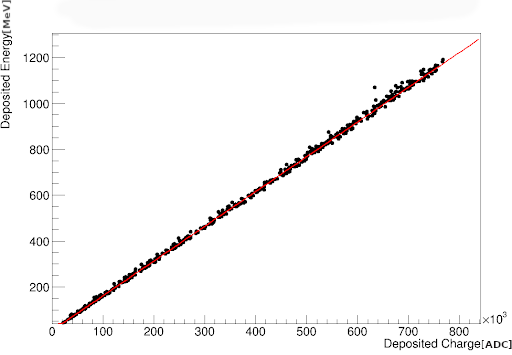
\includegraphics[width = 0.7\textwidth]{figures-chap4/linear_energy_lookup_curve1.png}
%    \captionsetup{type=figure}
%    \captionof{figure}{The linear relationship between deposited charge and energy. Produced from a sample of muons used for calibrating the \textit{Shower Linear Energy tool.}}
%    \label{fig:linear lookup curve}
%\end{center}
\newpage
\begin{figure}[h]
    \centering
    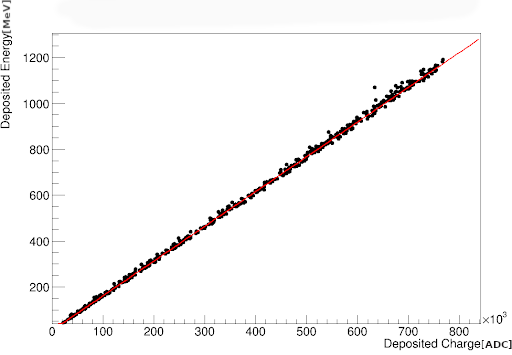
\includegraphics[width = \largefigwidth]{figures-chap4/linear_energy_lookup_curve1.png}
    \caption{The linear relationship between deposited charge and energy. Produced from a sample of muons used for calibrating the \textit{Shower Linear Energy tool.}}
    \label{fig:linear lookup curve}
\end{figure}



To estimate the reconstructed shower energy, the charge found to be associated with a shower would be used to directly read off the associated energy from the linear calibration. A further recombination correction is not required as it has already been accounted for in the charge to energy conversion. The fractional energy resolution of the \textit{Shower Linear Energy tool} is shown in \FigureRef{fig:linear_kGeVelectrons}. 

\subsection{Number of Electrons to Energy}\label{subchap:kGeVToElectrons}
The \textit{Shower Num Electrons Energy tool} was developed to move away from being reliant on in-house calibration curves and instead use the pre-existing calibration available in the \Gls{sbnd} portion of the \Gls{larsoft} framework. This has the advantage of being much more flexible to physics changes. For example a change in the recombination correction could be investigated by changing a single number, whereas, for the \textit{Linear Energy tool}, the calibration curves would have to be regenerated. The number of electrons are found from the \gls{adc} charge and are then directly converted to energy using a \textit{GeVToElectrons} scale factor which is the inverse of the energy required to ionise an argon atom. With this method a correction to account for recombination is still required. A nominal recombination value of 0.64 is used for all hits. 

The nominal recombination value was calculated by simulating electrons with a large (effectively infinite) lifetime and turning off any diffusion effects. The only thing remaining that may impact the collected energy is the recombination effect and therefore taking the ratio between the collected and deposited energy will give a value for the recombination value. For electrons, it was found that the recombination value was fairly constant at a value of 0.64 across a broad range of energies \cite{recombination_0.64}. 



\newpage
\begin{figure}[h]
    \centering
    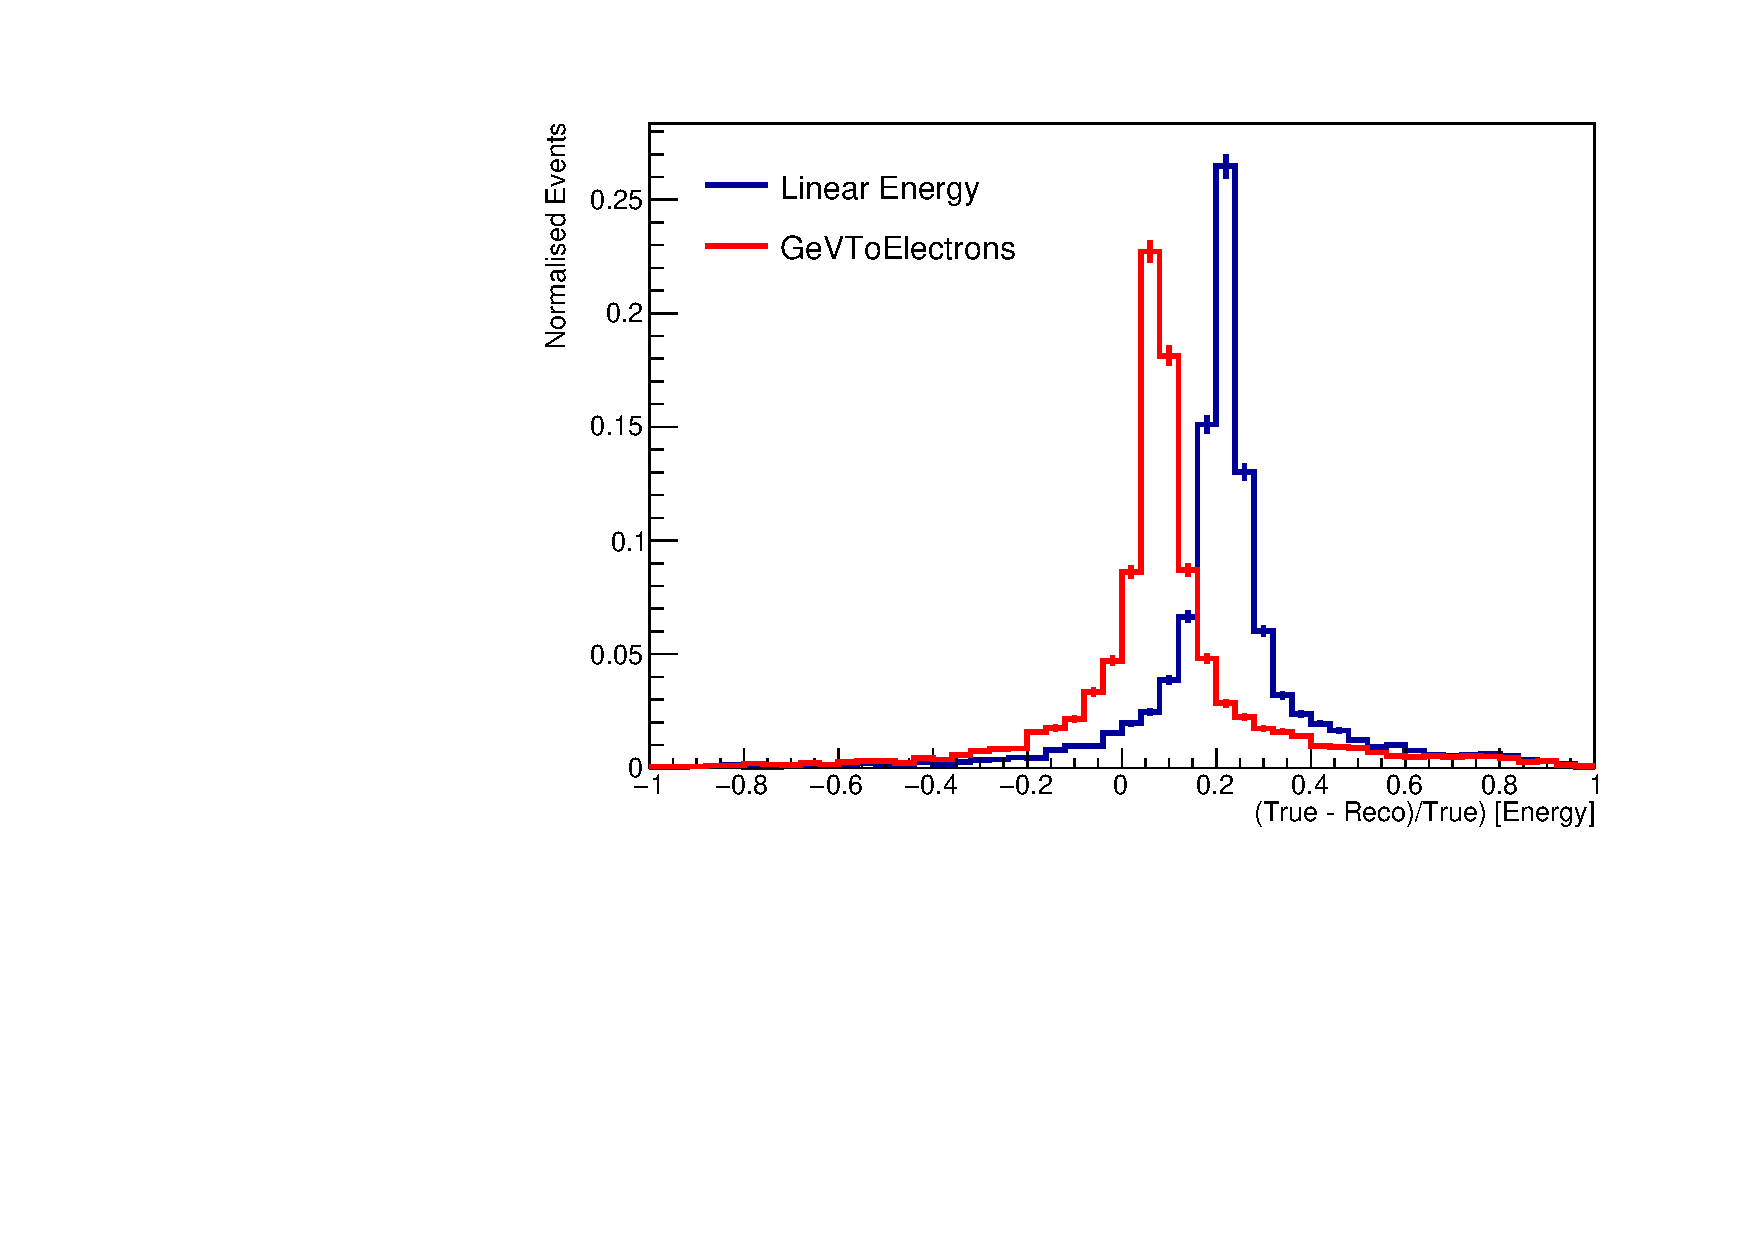
\includegraphics[width = \largefigwidth]{figures-chap4/linear_energy_kGeVElectrons_true_showering.pdf}
    \caption{Comparison of the \textit{Shower Linear Energy Tool} (Blue) and the \textit{Shower Num Electrons Energy Tool} (Red) with the true energy of the showering electrons.}
    \label{fig:linear_kGeVelectrons}
\end{figure}

\begin{comment}

An attempt to correct for the \Gls{sce} can be made with this method by utilising the Modified Box Recombination Model which is given by \begin{equation}\label{eqn:ModBox}
    \frac{dE}{dx} = \frac{\exp{(\frac{\beta}{\rho \mathcal{E}} W_{ion}.\frac{dQ}{dx}}) - \alpha}{\frac{\beta}{\rho \mathcal{E}}}
\end{equation}
where $\frac{dE}{dx}$ is the deposited energy per unit length, $\frac{dQ}{dx}$ is the deposited charge per unit length,  $\mathcal{E}$ is the electric field in the detector, $\rho$ is the density of liquid argon, $W_{ion} = 23.6$ eV which is the energy required to ionise an argon atom, $\alpha = 0.93 \pm 0.02$ and $\beta = 0.212 \pm 0.002$ (kV/cm)(g/cm$^2$)/MeV. The values for parameters $\alpha$ and $\beta$ are results from the \Gls{argoneut} experiment \cite{ArgoNeuT_recombination_paper}. The recombination correction, \textit{R} is given by $\frac{\frac{dQ}{dx}.W_{ion}}{\frac{dE}{dx}}$ and by taking the nominal values of \textit{R} and $\mathcal{E}$ a nominal value for $\frac{dE}{dx}$ is calculated using \EquationRef{eqn:ModBox}. Assuming the nominal value of $\frac{dE}{dx}$ is constant, \textit{R} may be expressed as $R = R(\mathcal{E}$). For each of the hits, their corresponding \Gls{sp} are found and the coordinates of the \Gls{sp} in the detector are determined. Instead of using the nominal value for $\mathcal{E}$, the local value for $\mathcal{E}$ at the position of the \Gls{sp} is used and the corresponding value for \textit{R} is calculated. The method to estimate the reconstructed energy is the same as the case without any \Gls{sce} corrections except the modified value for \textit{R} is used. In the case that a hit has no corresponding \Gls{sp}, the charge weighted centre of the shower is found and the local value of $\mathcal{E}$ at this point is used instead.

\begin{figure}[h]
    \centering
    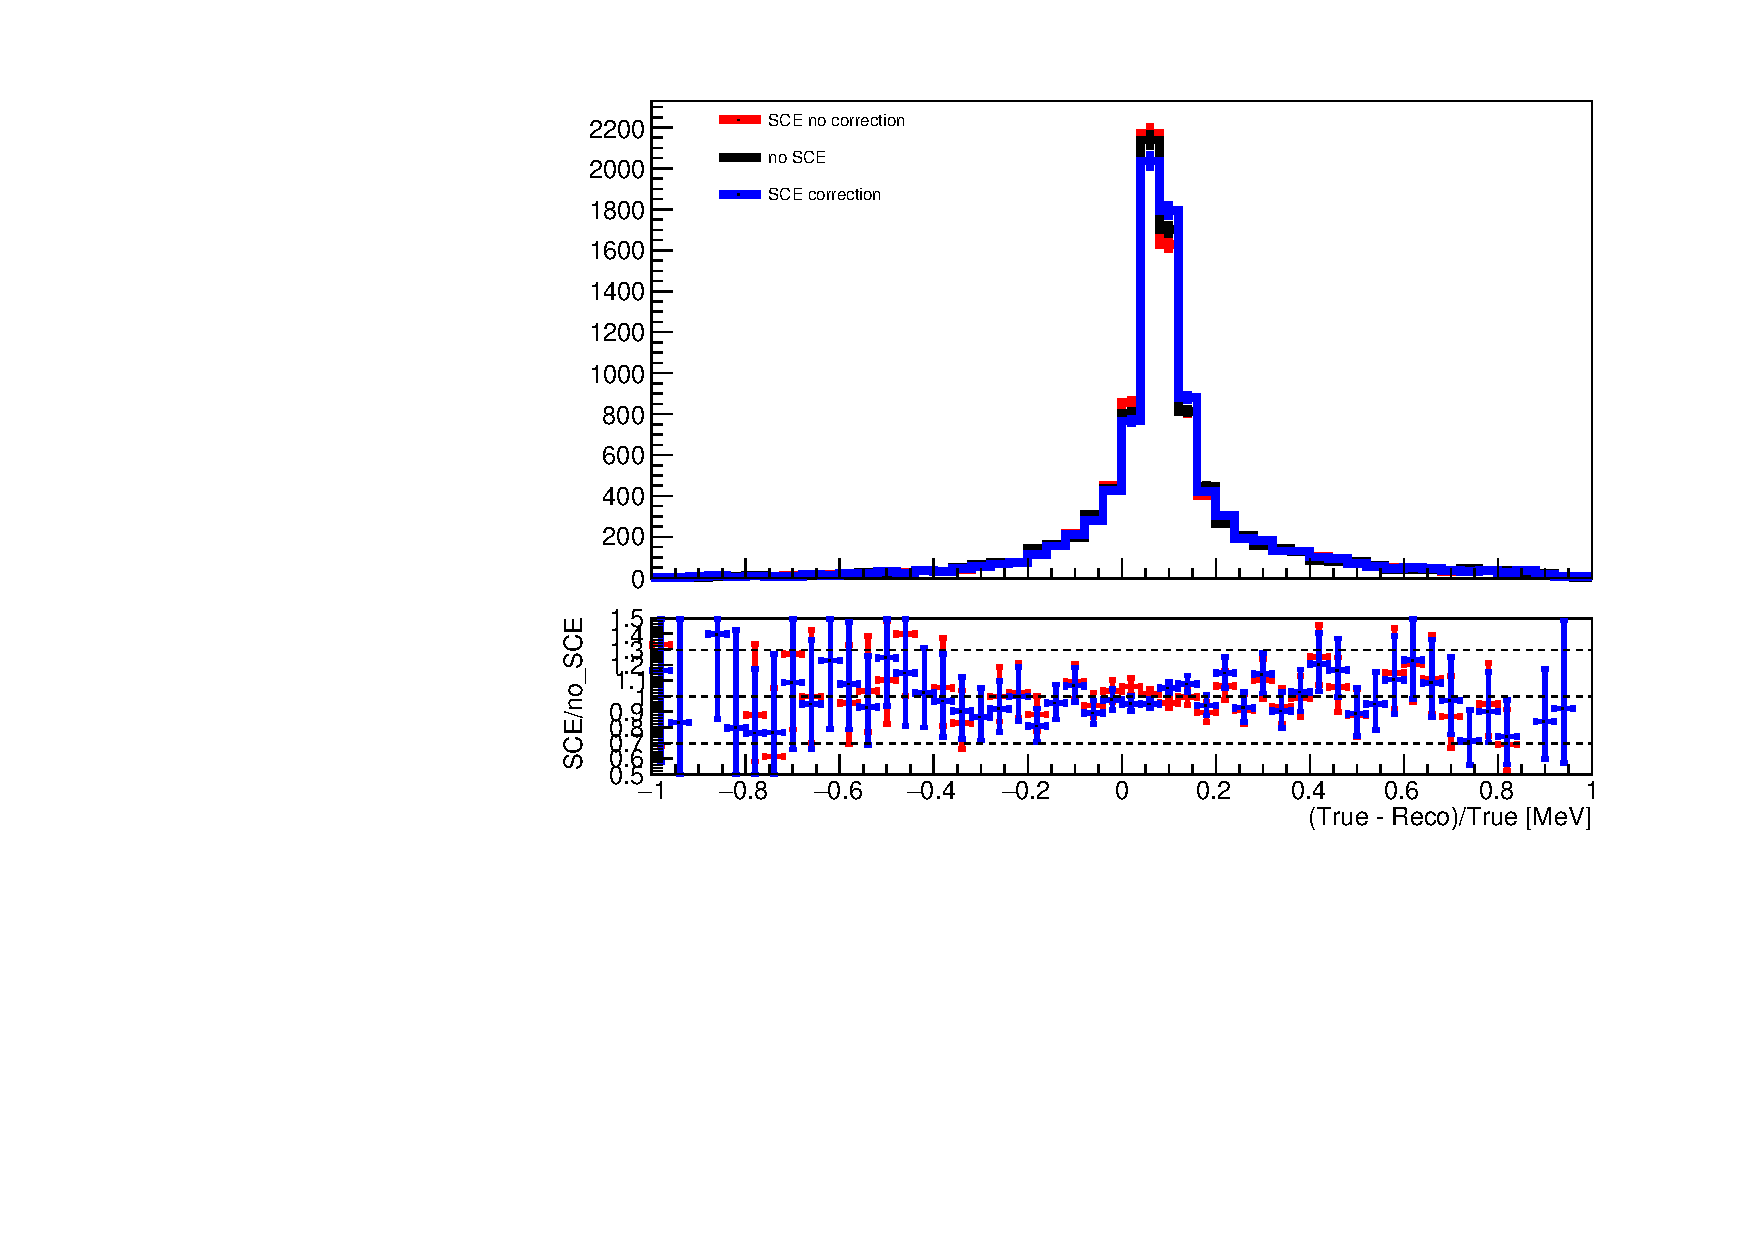
\includegraphics[width = \largefigwidth]{figures-chap4/ratio_plot_oldmethod_trueshoweringparticle.pdf}
    \caption{Caption}
    \label{fig:my_label}
\end{figure}



Shortcoming (don't know how much to put here? don't know if i want to emphasise how bad stuff is..): 
\begin{itemize}
    \item Things revolve around the nominal recomb of 0.64 - not really that realistic. 
    \item Correcting for SCE 'properly' is not straightforward either - using a fixed nominal dE/dx isn't ideal.
\end{itemize}

\end{comment}

\subsection{ESTAR Method}
The \textit{Shower ESTAR Energy tool} combines the ESTAR database provided by the \gls{nist} along with the Modified Box recombination model in an approach that was first used by the \Gls{argoneut} experiment \cite{ArgoNeuT_ESTAR_paper}. The ESTAR database provides the track length of electrons in various materials, including liquid argon, for energies ranging from 0.01 MeV to 1000 MeV \cite{ESTAR_Database}.

$\frac{dE}{dx}$ values may be calculated by dividing the energy by the track length for each entry in the ESTAR database. The deposited charge, \textit{Q}, can then found by using \EquationRef{eqn:ModBox} to find $\frac{dQ}{dx}$ and multiplying by the track length, \textit{dx}. This now allows the collected charge and energy to be related. If $\mathcal{E}$ in \EquationRef{eqn:ModBox} is taken to be a variable, the above process may be repeated whilst iterating over a set values of $\mathcal{E}$. This results in a 3D curve relating both the deposited charge and electric field to energy as is shown in \FigureRef{fig:ESTAR lookup curve}. The energy may then be interpolated from the collected charge and the appropriate electric field. As with the \textit{Linear Energy tool}, a direct correction for recombination isn't needed as it is again accounted for in the lookup curve. 

\begin{figure}[h]
    \centering
    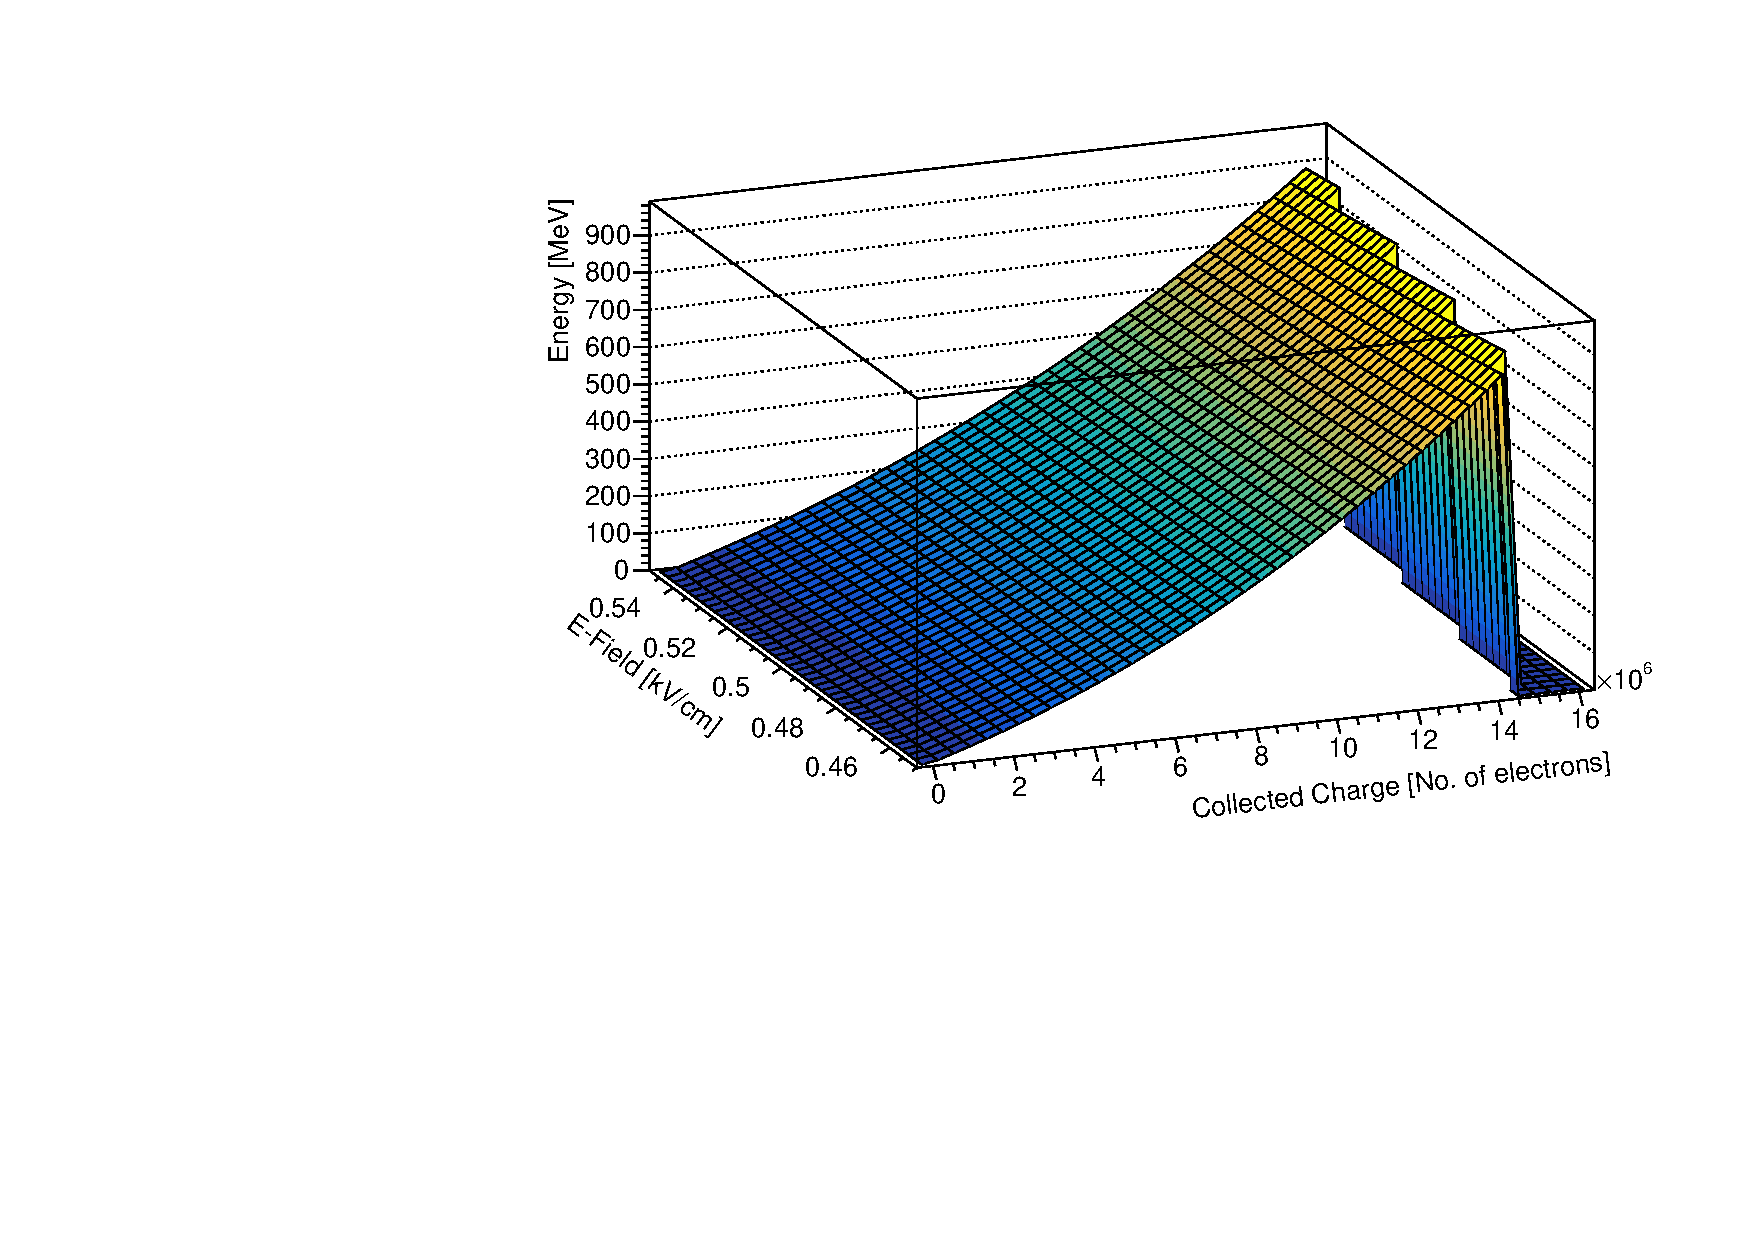
\includegraphics[width = 0.8\textwidth]{figures-chap4/ESTAR_lookup_curve.pdf}
    \caption{ESTAR Lookup Curve}
    \label{fig:ESTAR lookup curve}
\end{figure}

\section{Shower Energy Reconstruction Performance}



To assess the performance of the \textit{Shower ESTAR Energy tool}, the the reconstructed energy of each hit was summed up for all the hits in a shower. This was compared the sum of the true energy of all the hits.


\begin{figure}
    \centering
    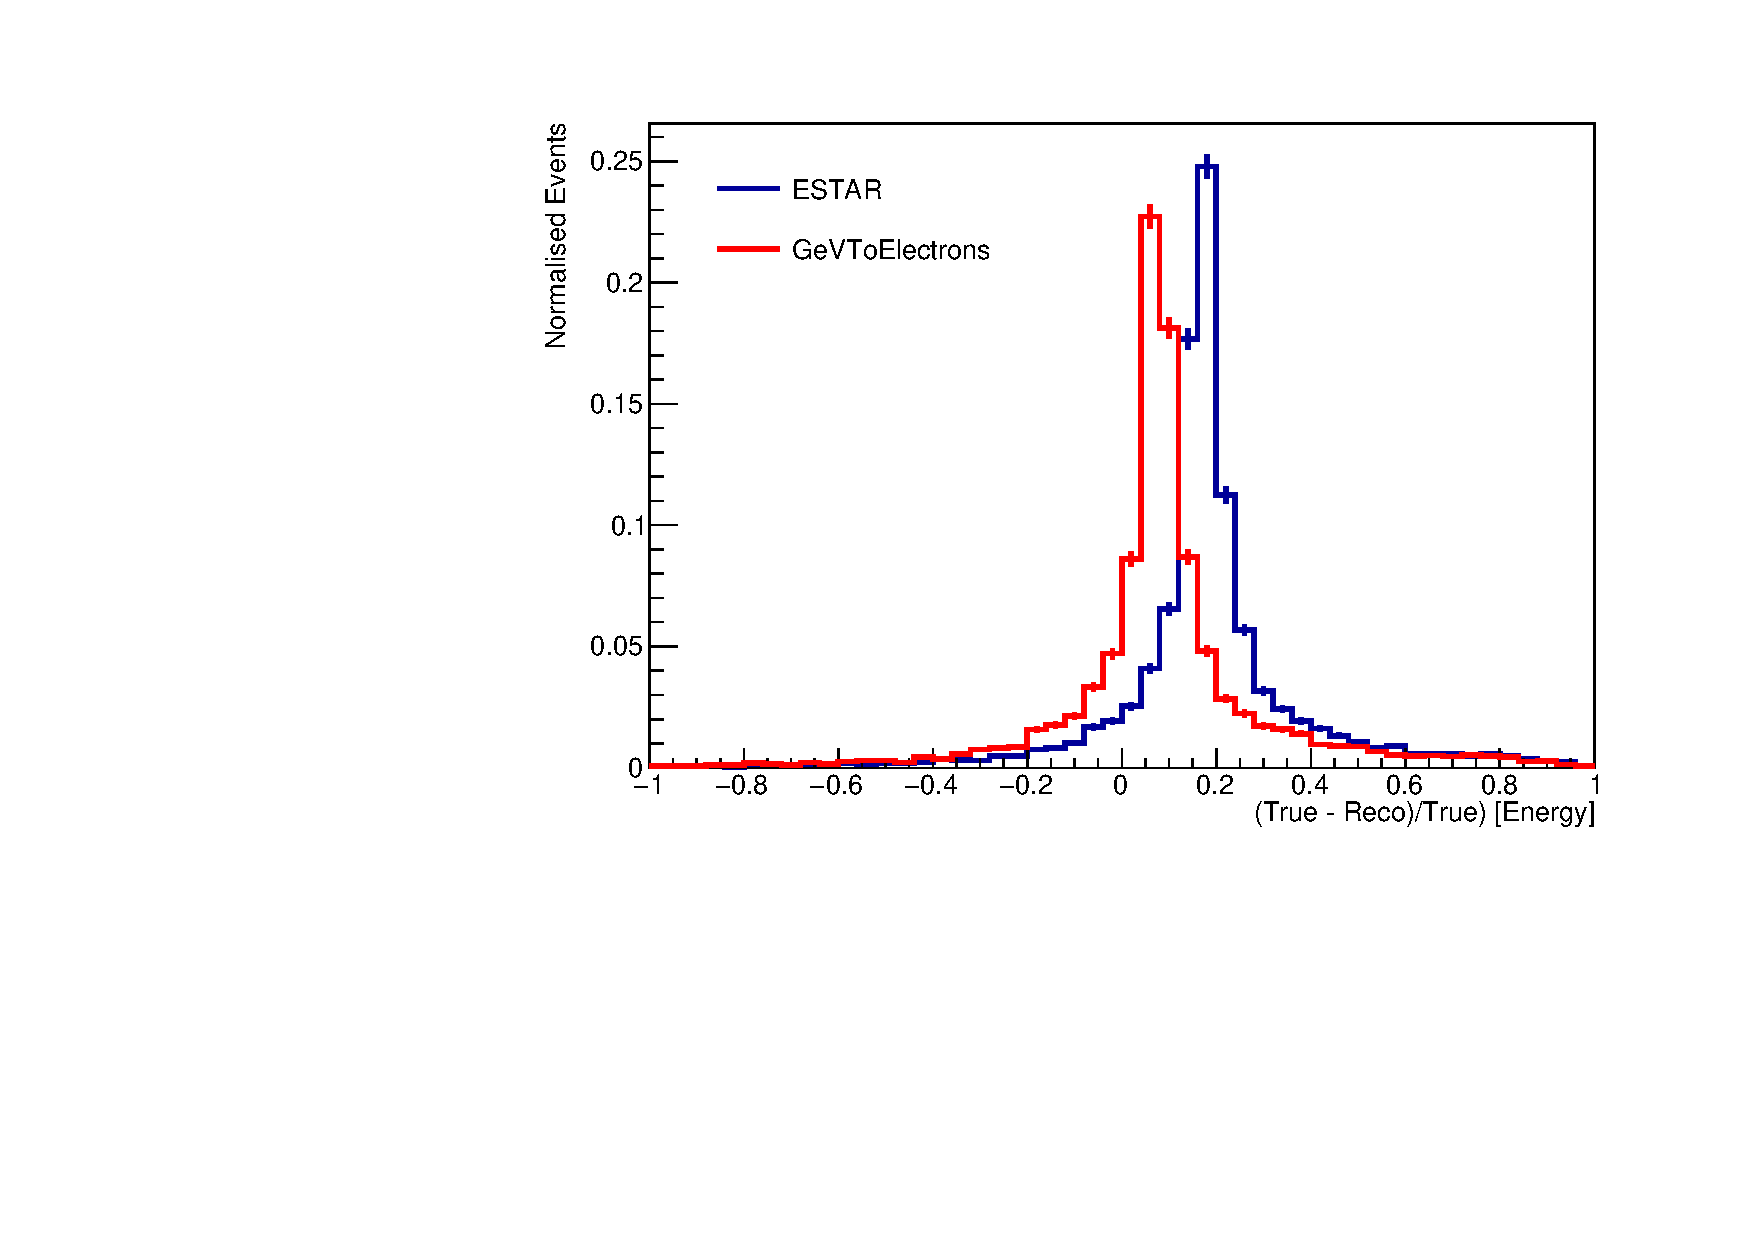
\includegraphics[width = \smallfigwidth]{figures-chap4/ESTAR_kGeVElectrons_true_showering.pdf}
    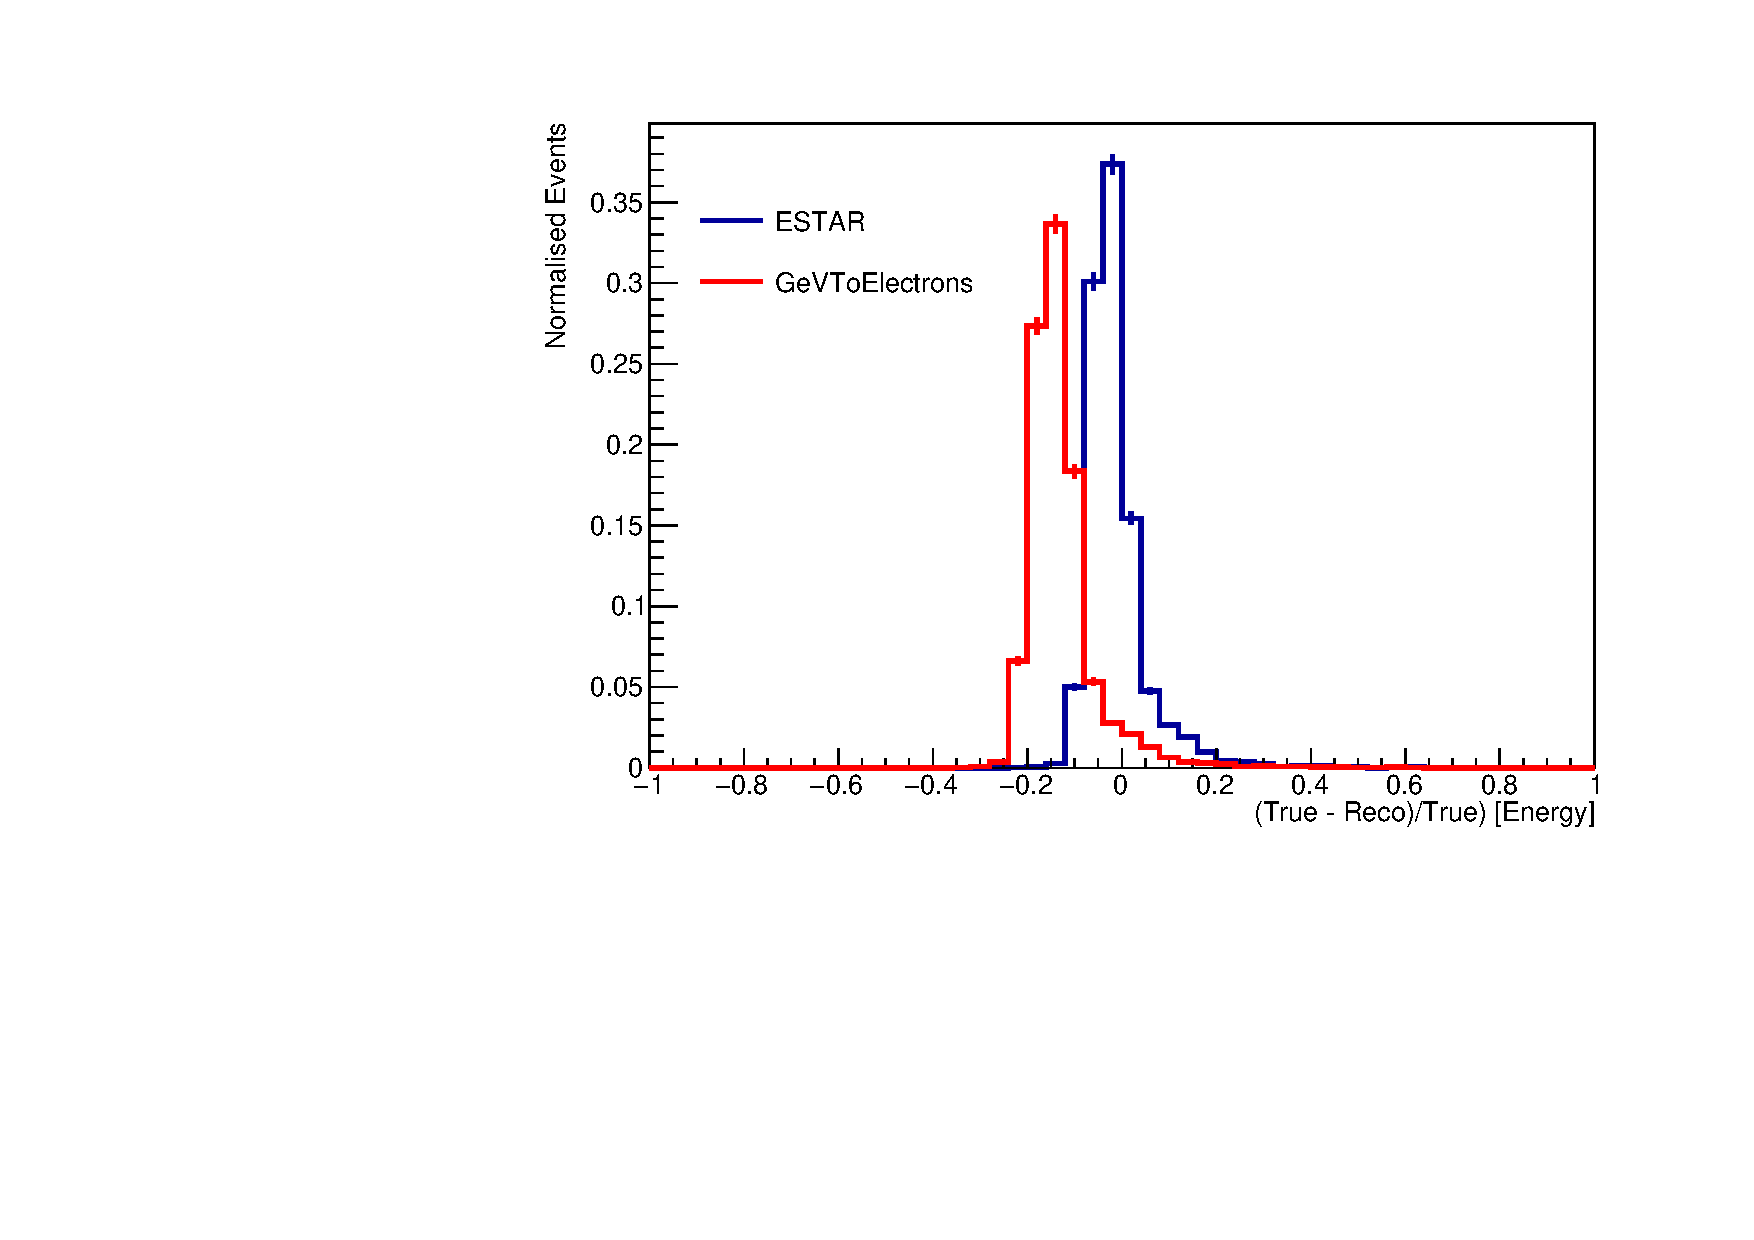
\includegraphics[width = \smallfigwidth]{figures-chap4/ESTAR_kGeVElectrons_true_hit.pdf}
    \caption{The fractional resolution of the \textit{Shower Num Electrons Energy Tool} and \textit{Shower ESTAR Energy Tool} compared with the true energy of the showering electron (left) and the sum of the true energy of all the hits (right). }
    \label{fig:my_label}
\end{figure}

\newpage
Other Validation stuff to do?
\begin{itemize}
    \item Use photon sample?
    \item validate for each individual plane and then best plane?
    \item Look at all showers in an event and compare with total showering energy. 
\end{itemize}


\section{Summary + outstanding issues etc}

Why getting dE/dx is hard (page 17).
Using muons as calibration
Energy bias corrections
https://inspirehep.net/files/f10063871db4836eb6ad935fcf761e7d

Energy Reco - Things to include.

\begin{itemize}
	\item Motivation (why do we care?)
	\item Explain choices - use vertex sample because it helps pandora. Only considering largest shower (most hits) from each event. 
	\item Overview of the very first method that was being used. Use muons to generate lookup curve. Get linear relationship between deposited charge and energy. Plagiarise Dom's thesis on this..  
	\item Change method so we convert the deposited charge to number of electrons and then convert the number of electrons to energy using the appropriate calibration/scale factors. Apply correction for electron lifetime as before and also correct for recombination. Previously recombination correction was 'baked' into the look-up curve. No way to correct for it directly - whenever we would change the \textit{physics} we would need to regenerate the look-up curve. With this method it's possible to tweak the recombination correction directly. 
	\item Not straight forward to calculate the recombination directly - let's use and average value for all showers - explain recombination study. 
	\item Consider SCE - explain what SC is.
	\item How do we account for SCE? Get map of the E-field in the detector (not uniform because of SC). Using the nominal value of the recombination and E-field, calculate a nominal dE/dx (not straightforward to calculate directly) which we assume remains constant. Can now use the Modified Box model to weak the recombination correction by feeding the local E-field (which depends on the location in the detector) back into the modified box model. Finally, find the (charge weighted) centre of the shower using the space points and use the local E-field at this point to calculate the recombination factor at this location. 
	\item No reason we can't do a per-hit analysis. Redo everything as before for each individual hit and then sum to get the energy of the shower. Should give better results since the recombination correction is more accurate now. 
	\item We have the ability to attempt to correct for the SCE as mentioned, but are limited by not knowing the dE/dx. So correcting the SCE without this caveat becomes tricky.. Try a new approach developed by ArgoNeuT - use the ESTAR database. The ESTAR database gives us the stopping power of (dE/dx) of electrons in various materials (including lAr) in a range of energies and is based partly from data. Combining this with the modified box recombination model, we can again create a lookup curve of energy vs deposited charge with the recombination correction baked in. Since the modified box model depends on the E-Field, we can treat this as a variable and create a 3D lookup curve of energy vs E-Field vs deposited charge which will allow us to correct for SC. 
	\item \textit{True} energy debacle.. We have the true energy of the showering particle and the true energy of all the hits in a given shower. Originally we used the true energy of the showering particle for comparison (in hindsight this seems like a stupid idea..) and the kGeVtoElectrons method clearly outperformed ESTAR. Swapping to the true hit energies, ESTAR does better. What was happening (i think) is that kGeVToElectrons over estimates the hit energies, so when comparing with the true showering particle this method give a better result because we're papering over the cracks due to the pattern recognition and hit inefficiencies. ESATR method gives a better result for individual hit energies so highlights the failing of the patter rec and hit inefficiencies when comparing with the showering particle. 
	\item Why some results are shit.. Pandora pattern recognition (clustering) is far from perfect - can use Pandora in cheating mode to overcome this. There are hit inefficiencies i.e. hit reconstruction isn't perfect - haven't ever \textit{cheated} this, dunno if it's an option. The actual impact from SC is pretty minimal but it also impacts Pandora's pattern recognition. This can a have a big impact - what Pandora initially recognised as one big shower may be interpreted as 2+ smaller showers after applying SC (and vice-versa). Also, an object classified as a shower may instead be classified as a track after applying SC. Since we're only considering the largest shower for each event, this effects mean SC can appear to have a impact. 
\end{itemize}

  %\chapter{VALOR Analysis}
\label{chap:VALOR}

Keep numu section? Perhaps too much overlap with Rhiannon's stuff.

\section{VALOR Framework}
\section{\texorpdfstring{$\nu_\mu$ and $\nu_e$ Selections}{numu and nue Selections}}
Link in with Energy Reco. section
\section{Flux Systematics}
\section{Interaction Systematics}
\section{Other Systematics}
MEC and POT
\section{\texorpdfstring{$\nu_\mu$ Disappearance Analysis}{numu Disappearance Analysis}}
\section{\texorpdfstring{$\nu_e$ Appearance Analysis}{nue Appearance Analysis}}
\section{\texorpdfstring{$\nu_e$ Disappearance Analysis}{nue Disappearance Analysis}}
\section{Additional Efficiency and Energy Scale Systematics}


Plots to include
\begin{itemize}
    \item Spline validation plots + tick table (will need to 'make these look good')
    \item Standard spectra x3
    \item Spectra with error envelopes (will need some work - think this was a pain cos have to force osc params so the osc sample is actually used.)
    \item Spectra (ratios) with various oscillation params ala tech note.
    \item contribution to sensitivity from each detector + detector combos.
    \item Contribution from each systematic group.
    \item Impact of various detector systematics 
    \item Standard exclusion/allowed sensitivities with all systematics (pick some value for the detector syst).
    \item Sensitivities with external limits.
\end{itemize}
  %\chapter{Conclusion}
\label{chap:Conclusion}
  %% To ignore a specific chapter while working on another, making the build faster, comment it out:
  %\input{chap4}
\end{mainmatter}

%% Produce the appendices
\begin{appendices}
  %% The "\appendix" call has already been made in the declaration
%% of the "appendices" environment (see thesis.tex).
\chapter{Pointless extras}
\label{app:Pointless}

\chapter{Some more stuff}

%% Big appendixes should be split off into separate files, just like chapters
%\input{app-myreallybigappendix}

\end{appendices}

%% Produce the un-numbered back matter (e.g. colophon,
%% bibliography, tables of figures etc., index...)
\begin{backmatter}
  \begin{colophon}
  This thesis was made in \LaTeXe{} using the ``hepthesis'' class.
\end{colophon}

%% You're recommended to use the eprint-aware biblio styles which
%% can be obtained from e.g. www.arxiv.org. The file mythesis.bib
%% is derived from the source using the SPIRES Bibtex service.
\bibliographystyle{h-physrev}
\sloppy
\bibliography{mythesis}



%% If you have time and interest to generate a (decent) index,
%% then you've clearly spent more time on the write-up than the 
%% research ;-)
%\printindex

%\chapter{Likely Examiner Questions}\label{Likely Examiner Questions}

After having read parts of the thesis, these are some of the questions people think are likely to come up in the viva. Don't necessarily need to include an explanation in the text, but should be prepared to answer.

\begin{itemize}
    \item Background/Theory
    \begin{itemize}
        \item Brief description / be able to sketch the historically significant neutrino experiments.
    \end{itemize}
    
    \item SBN Programme
    \begin{itemize}
        \item Energy threshold calculation for nue, numu, nutau interaction. (see https://www.hep.phy.cam.ac.uk/~thomson/partIIIparticles/handouts/Handout\_11\_2011.pdf)
    \end{itemize}
    
    \item Energy Reco
    \begin{itemize}
        \item "Apply signal processing techniques" - what are these techniques?
        \item Why the deconvolved charge drops below 0?
        \item Explanation for the resolution comparisons. Linear and ESTAR pretty close - I think this may just be a binning artefact. Num Electrons a little wider - it systematically assigns higher energies to the hits, so the spread in energies will also be a little broader hence the wider fit. 
    \end{itemize}
    
    \item VALOR
    \begin{itemize}
        \item Understand the origin of the dominant systematics + how they are modelled. 
        \item Why do the injected contours look janky (stat/syst lines cross?) Don't know.. But have seen this many times + other fitters all see weirdness.. Feels like the fit has a real problem "closing" the contour.  
    \end{itemize}
\end{itemize}


\end{backmatter}




%% Close
\end{document}
